% meta.concepts: 2D moment
% meta.tags: realistic
% acknowledge: Peter Seiler & Luke Melander graciously shared Spring 2019 course material
% source: 2019 P. Seiler AEM2011 HW 3

A 75 kilogram tightrope walker is attempting a walk across a 50 meter span 20 meters above the ground. When
he is 20\% across the span, the rope is deflected such that he is 17 meters above the ground. Find the tension
in the rope both ahead of and behind the walker, and the moments about points A and B (where the support
posts meet the ground). Ignore the mass of the rope itself.


\begin{figure}[ht!]
  \centering
  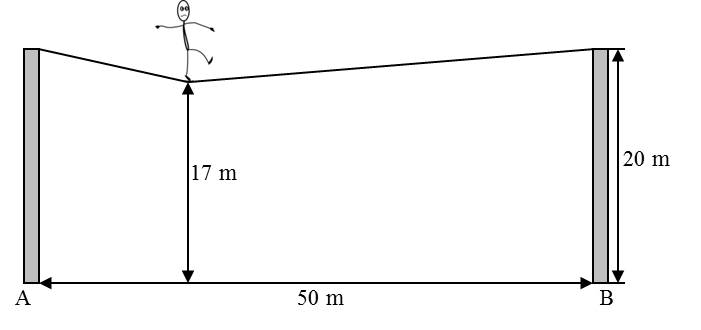
\includegraphics[height=1.8in]{fig.png}
\end{figure}

\iftoggle{flagSoln}{%
\vspace{.5cm}
\rule{\textwidth}{.4pt}
\vspace{.5cm}
\textbf{Solution:}
\begin{figure}[ht!]
  \centering
  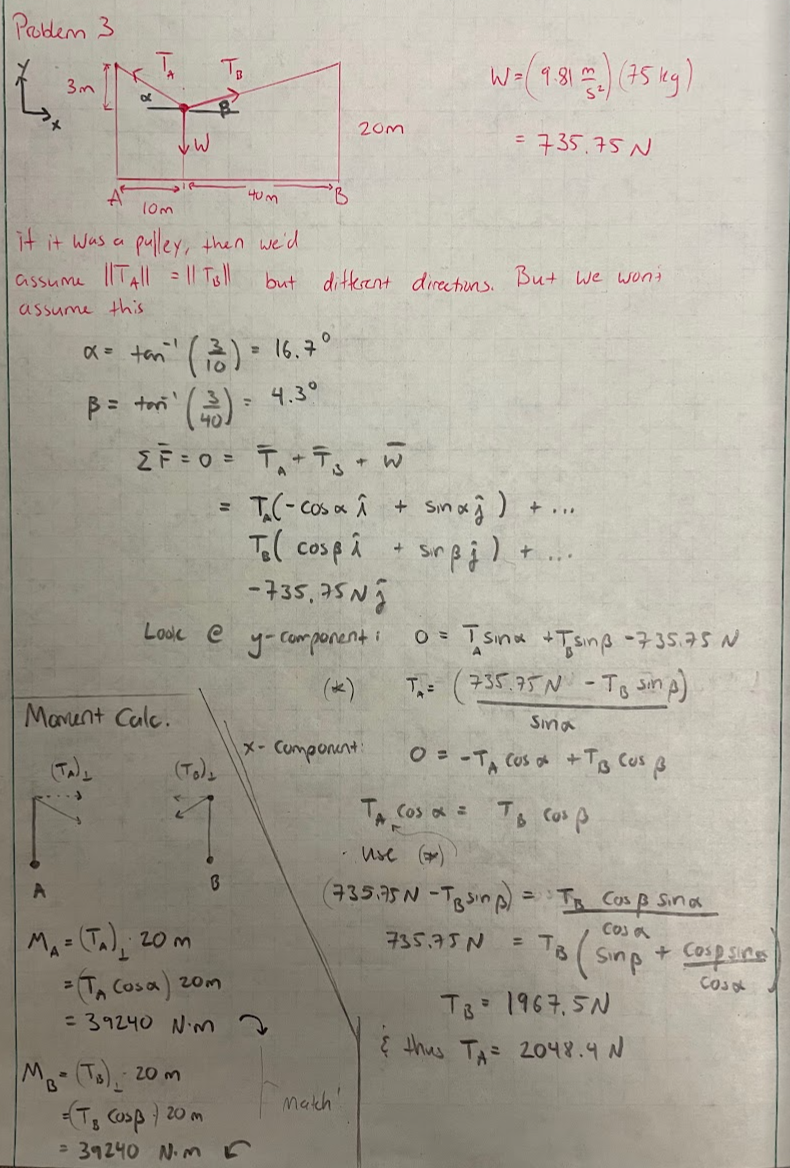
\includegraphics[width=0.9\textwidth,
	           height=0.3\textheight,
		   keepaspectratio]{soln.png}
\end{figure}
}{%
}%
